En una ciutat s'ha estudiat la relació entre els hàbits de lectura i la pràctica d'esport en l'alumnat de
batxillerat. Per a fer-ho, s'han formulat les dues preguntes següents a l'alumnat d'aquesta etapa
educativa: «Llegeixes com a mínim dos llibres al mes?» i «Practiques algun esport almenys quatre hores a
la setmana?»

Dels resultats de l'enquesta, es desprèn que el 60\,\% llegeixen com a mínim dos llibres al mes, dels quals
el 70\,\% practiquen algun esport un mínim de quatre hores a la setmana. També s'observa que, d'entre els que
no llegeixen un mínim de dos llibres al mes, el 50\,\% fan menys de quatre hores setmanals d'esport.

Si escollim a l'atzar un alumne/a de batxillerat d'aquesta ciutat:

\begin{apartats}

\apartat{0,75}
Quina és la probabilitat que faci esport almenys quatre hores setmanals?

\begin{solucio}
Considerem els successos aleatoris següents: $Ll$ = «llegir almenys dos llibres al mes» i $E$ = «fer un
mínim de quatre hores setmanals d'esport». Les dades del problema ens diuen que $P(Ll)=0{,}6$,
$P(E\mid Ll)=0{,}7$ i $P\bigl(\overline{E}\mid\overline{Ll}\bigr)=0{,}5$. Podem visualitzar-les en el diagrama
d'arbre adjunt:
\begin{center}
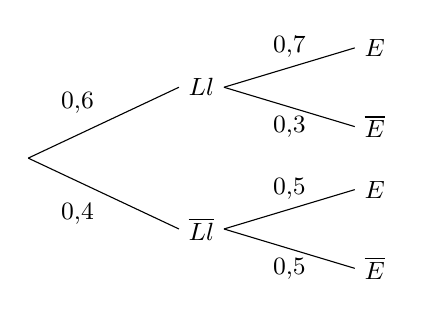
\begin{tikzpicture}[x=1cm,y=1cm,font=\small]
  \coordinate (o) at (0,0);
  \node (L) at (2.2,0.9) {$Ll$};
  \node (N) at (2.2,-0.9) {$\overline{Ll}$};
  \draw (o) -- node[above left]{$0{,}6$} (L.west);
  \draw (o) -- node[below left]{$0{,}4$} (N.west);
  \node (LE) at (4.4,1.4) {$E$};  \node (LN) at (4.4,0.4) {$\overline{E}$};
  \node (NE) at (4.4,-0.4) {$E$}; \node (NN) at (4.4,-1.4) {$\overline{E}$};
  \draw (L.east) -- node[above]{$0{,}7$} (LE.west); \draw (L.east) -- node[below]{$0{,}3$} (LN.west);
  \draw (N.east) -- node[above]{$0{,}5$} (NE.west); \draw (N.east) -- node[below]{$0{,}5$} (NN.west);
\end{tikzpicture}
\end{center}
Pel teorema de la probabilitat total,
\[
P(E)=P(Ll)\cdot P(E\mid Ll)+P\bigl(\overline{Ll}\bigr)\cdot P\bigl(E\mid\overline{Ll}\bigr)
=0{,}6\cdot0{,}7+0{,}4\cdot0{,}5=0{,}42+0{,}20=0{,}62 .
\]

\textit{Pauta oficial:} 0,25 per plantejar la llei de la probabilitat total, 0,25 per identificar les dades
del problema i 0,25 pel càlcul.
\end{solucio}

\apartat{0,75}
Si sabem que aquest alumne/a fa esport menys de quatre hores setmanals, quina probabilitat hi ha que llegeixi
almenys dos llibres al mes?

\begin{solucio}
Per la fórmula de Bayes,
\[
P\bigl(Ll\mid\overline{E}\bigr)=\frac{P\bigl(Ll\cap\overline{E}\bigr)}{P\bigl(\overline{E}\bigr)}
=\frac{P\bigl(\overline{E}\mid Ll\bigr)\cdot P(Ll)}{1-P(E)}=\frac{0{,}3\cdot0{,}6}{1-0{,}62}=0{,}47\ldots
\]

\textit{Pauta oficial:} 0,25 per plantejar la fórmula de Bayes (o la fórmula de la probabilitat
condicionada) i 0,5 pel càlcul.
\end{solucio}

\apartat{1}
L'Alba és una estudiant de batxillerat que ha anat anotant durant tot el curs quantes hores dedicava a la
setmana a llegir i quantes a fer esport. Per a cada setmana té apuntat un nombre real $x$ que correspon a la
quantitat d'hores de lectura i que oscil·la entre 1 i 6, i un nombre real $y$ que correspon a la quantitat
d'hores de pràctica esportiva. Ha observat que la relació $y=7-x+\ln(2x-1)$ s'ajusta força bé a les dades
que ha anotat.

Calculeu, segons aquest model, quin és el màxim i el mínim d'hores per setmana que l'Alba ha dedicat a
practicar esport.

\begin{solucio}
Cal trobar els valors màxim i mínim absoluts de la funció $f(x)=7-x+\ln(2x-1)$ a l'interval $[1,6]$. La
derivada de $f(x)$ és $f'(x)=-1+\dfrac{2}{2x-1}$, que s'anul·la només per a $x=\frac32$. Aquest punt crític
es correspon amb un màxim local, ja que la funció (a la vista del signe de la derivada) creix per a
$x<\frac32$ i decreix per a $x>\frac32$. Com que $f(1)=7-1+\ln1=6$, $f\!\left(\frac32\right)=7-\frac32+\ln2
\approx6{,}19$ i $f(6)=7-6+\ln11\approx3{,}4$, deduïm que el màxim i el mínim absoluts de la funció a
l'interval $[1,6]$ són els punts $f\!\left(\frac32\right)\approx6{,}19$ i $f(6)\approx3{,}4$, respectivament.
Per tant, segons aquest model, l'Alba ha practicat entre un mínim de 3,4 i un màxim de 6,19 hores per
setmana d'esport.

\textit{Pauta oficial:} 0,25 per la derivada i per detectar que $\frac32$ és l'únic punt crític, 0,25 per
les zones de creixement i decreixement, 0,25 per argumentar el màxim global i 0,25 per argumentar el mínim
global.
\end{solucio}

\end{apartats}
